%%%%%%%%%%%%%%%%%%%%%%%%%%%%%%%%%%%%%%%%%%%%%%%%%%%%%%%%%%%%%%%%%%%%%
%%                                                                 %%
%% Please do not use \input{...} to include other tex files.       %%
%% Submit your LaTeX manuscript as one .tex document.              %%
%%                                                                 %%
%% All additional figures and files should be attached             %%
%% separately and not embedded in the \TeX\ document itself.       %%
%%                                                                 %%
%%%%%%%%%%%%%%%%%%%%%%%%%%%%%%%%%%%%%%%%%%%%%%%%%%%%%%%%%%%%%%%%%%%%%

%%\documentclass[referee,sn-basic]{sn-jnl}% referee option is meant for double line spacing

%%=======================================================%%
%% to print line numbers in the margin use lineno option %%
%%=======================================================%%

%%\documentclass[lineno,sn-basic]{sn-jnl}% Basic Springer Nature Reference Style/Chemistry Reference Style

%%======================================================%%
%% to compile with pdflatex/xelatex use pdflatex option %%
%%======================================================%%

%%\documentclass[pdflatex,sn-basic]{sn-jnl}% Basic Springer Nature Reference Style/Chemistry Reference Style

%%\documentclass[sn-basic]{sn-jnl}% Basic Springer Nature Reference Style/Chemistry Reference Style
\documentclass[sn-mathphys]{sn-jnl}% Math and Physical Sciences Reference Style
%%\documentclass[sn-aps]{sn-jnl}% American Physical Society (APS) Reference Style
%%\documentclass[sn-vancouver]{sn-jnl}% Vancouver Reference Style
%%\documentclass[sn-apa]{sn-jnl}% APA Reference Style
%%\documentclass[sn-chicago]{sn-jnl}% Chicago-based Humanities Reference Style
%%\documentclass[sn-standardnature]{sn-jnl}% Standard Nature Portfolio Reference Style
%%\documentclass[default]{sn-jnl}% Default
%%\documentclass[default,iicol]{sn-jnl}% Default with double column layout

%%%% Standard Packages
%%<additional latex packages if required can be included here>
%%%%

%%%%%=============================================================================%%%%
%%%%  Remarks: This template is provided to aid authors with the preparation
%%%%  of original research articles intended for submission to journals published 
%%%%  by Springer Nature. The guidance has been prepared in partnership with 
%%%%  production teams to conform to Springer Nature technical requirements. 
%%%%  Editorial and presentation requirements differ among journal portfolios and 
%%%%  research disciplines. You may find sections in this template are irrelevant 
%%%%  to your work and are empowered to omit any such section if allowed by the 
%%%%  journal you intend to submit to. The submission guidelines and policies 
%%%%  of the journal take precedence. A detailed User Manual is available in the 
%%%%  template package for technical guidance.
%%%%%=============================================================================%%%%

\jyear{2021}%

%% as per the requirement new theorem styles can be included as shown below
\theoremstyle{thmstyleone}%
\newtheorem{theorem}{Theorem}%  meant for continuous numbers
%%\newtheorem{theorem}{Theorem}[section]% meant for sectionwise numbers
%% optional argument [theorem] produces theorem numbering sequence instead of independent numbers for Proposition
\newtheorem{proposition}[theorem]{Proposition}% 
%%\newtheorem{proposition}{Proposition}% to get separate numbers for theorem and proposition etc.

\theoremstyle{thmstyletwo}%
\newtheorem{example}{Example}%
\newtheorem{remark}{Remark}%
\theoremstyle{thmstylethree}%
\newtheorem{definition}{Definition}%
\usepackage{url}
\usepackage{hyperref}
\usepackage{adjustbox}
\raggedbottom
%%\unnumbered% uncomment this for unnumbered level heads

\begin{document}

\title[Article Title]{Parabolic Depth Estimation from Image Blur Using Tenengrad Scores with a Single RGB Camera}

%%=============================================================%%
%% Prefix	-> \pfx{Dr}
%% GivenName	-> \fnm{Joergen W.}
%% Particle	-> \spfx{van der} -> surname prefix
%% FamilyName	-> \sur{Ploeg}
%% Suffix	-> \sfx{IV}
%% NatureName	-> \tanm{Poet Laureate} -> Title after name
%% Degrees	-> \dgr{MSc, PhD}
%% \author*[1,2]{\pfx{Dr} \fnm{Joergen W.} \spfx{van der} \sur{Ploeg} \sfx{IV} \tanm{Poet Laureate} 
%%                 \dgr{MSc, PhD}}\email{iauthor@gmail.com}
%%=============================================================%%

\author[1]{\fnm{Divakar} \sur{Keshri}}\email{keshri9@gmail.com}

\author[2]{\fnm{K.V.} \sur{Sriharsha}}\email{sriharsha.phd@gmail.com}
%\equalcont{These authors contributed equally to this work.}

\author*[3]{\fnm{P.J.A} \sur{Alphonse}}\email{alphonse@nitt.edu}
%\equalcont{These authors contributed equally to this work.}

\affil[1]{\orgdiv{Department of Computer Applications}, \orgname{National Institute of Technology
}, \orgaddress{\street{} \city{Tiruchirappalli}, \postcode{620015}, \state{Tamilnadu}, \country{India}}}

\affil[2]{\orgdiv{Department of Automation  }, \orgname{OLA Electric Technologies Private Limited (OLA\_OET)
}, \orgaddress{\street{}\city{Bengaluru}, \postcode{560095}, \state{Karnataka }, \country{India}}}

%%==================================%%
%% sample for unstructured abstract %%
%%==================================%%

\abstract{Depth estimation is a crucial task in computer vision, with 
applications in robotics, augmented reality, and autonomous vehicles. 
This study presents a novel method for estimating depth from a single 
RGB image by leveraging the Tenengrad score, a focus measure operator, 
to quantify image blurriness relative to focus distance. By adjusting 
the aperture and moving the object towards and away from predefined 
focus distances, we capture images at varying levels of blurriness. 
The Tenengrad score, computed from the gradients in the x and y 
directions, quantifies these blur variations. Using these scores, 
along with focus and aperture settings, we train a Random Forest 
Regressor to predict object distances within the range of 0.25m to 
1.1m. An updated dataset of 393 real-time photos, captured using a 
DSLR camera and paired with ground truth depth information obtained 
from a laser distance meter, is introduced. Our experiments 
demonstrate a parabolic relationship between depth and blurriness, 
achieving high correlation (r=0.9999) and negligible RMSE 
$(8.604584927025298 \times 10^{-13})$ in depth estimation.
}
%%================================%%
%% Sample for structured abstract %%
%%================================%%

% \abstract{\textbf{Purpose:} The abstract serves both as a general introduction to the topic and as a brief, non-technical summary of the main results and their implications. The abstract must not include subheadings (unless expressly permitted in the journal's Instructions to Authors), equations or citations. As a guide the abstract should not exceed 200 words. Most journals do not set a hard limit however authors are advised to check the author instructions for the journal they are submitting to.
% 
% \textbf{Methods:} The abstract serves both as a general introduction to the topic and as a brief, non-technical summary of the main results and their implications. The abstract must not include subheadings (unless expressly permitted in the journal's Instructions to Authors), equations or citations. As a guide the abstract should not exceed 200 words. Most journals do not set a hard limit however authors are advised to check the author instructions for the journal they are submitting to.
% 
% \textbf{Results:} The abstract serves both as a general introduction to the topic and as a brief, non-technical summary of the main results and their implications. The abstract must not include subheadings (unless expressly permitted in the journal's Instructions to Authors), equations or citations. As a guide the abstract should not exceed 200 words. Most journals do not set a hard limit however authors are advised to check the author instructions for the journal they are submitting to.
% 
% \textbf{Conclusion:} The abstract serves both as a general introduction to the topic and as a brief, non-technical summary of the main results and their implications. The abstract must not include subheadings (unless expressly permitted in the journal's Instructions to Authors), equations or citations. As a guide the abstract should not exceed 200 words. Most journals do not set a hard limit however authors are advised to check the author instructions for the journal they are submitting to.}

\keywords{Aperture Number, f-stop, Tenengrad (Tenegrad), Exposure Time, Film Speed, Focal Length, focus, aperture, RMSE, MAE.}

%%\pacs[JEL Classification]{D8, H51}

%%\pacs[MSC Classification]{35A01, 65L10, 65L12, 65L20, 65L70}

\maketitle
\section{Introduction}\label{sec1}

A. Motivation: \par
Image depth estimation, also known as depth inference or prediction, is a crucial computer vision task used in robotics, augmented reality, and driver-less vehicles. In this case, estimating depth from blur is helpful, particularly when working with out-of-focus objects. As a result, focus measure operators serve as a practical and efficient proxy for blur when assessing an image's sharpness or clarity\par

This work attempts to estimate the depth from an out-of-focus image, which ultimately depends on the blur factor. To achieve this, we intend to compute the gradients using the gradient focus measure. Next, we'll determine the degree of blur by looking at the textures in the blurred area and the gradient's intensity on the highlighted boundaries.\par

Sharp images \cite{bib1} have well-defined edges and high contrast between adjacent pixels. The Sobel operator, used in the \textbf{Tenengrad} focus measure, detects these edges by computing the gradient magnitude at each pixel. Similarly, Blurred images have smoother transitions between adjacent pixels, resulting in lower contrast and less pronounced edges. The gradients in these areas will have lower magnitudes.  The Sobel operator used in \textbf{Tenengrad} is less sensitive to a sharp image, edges and fine details are prominent, resulting in high gradient magnitudes. Thus, the tenengrad score will be higher.  In a blurry image, edges, and details are smoothed out, leading to lower gradient magnitudes. Consequently, the tenengrad score will be lower. Thus, there is an inverse relationship between blurriness and the tenengrad score: noise compared to other high-pass filters like the Laplacian and is computationally efficient, making it suitable for real-time applications.\par

 

B. Research Contributions:
\begin{itemize}
  \item Exploring the relationship between the Tenengrad score and blurriness in the image. 

  \item Quantifying the amount of blurriness in the image w.r.t to the focal distance using the Tenengrad score.

  \item A parabolic (quadratic) model to describe the relationship between depth and blurriness.

  \item Influence of Predicted distance on Tenengrad score for different focus settings
  
\end{itemize}


The structure of the manuscript's body is as follows: The literature review is provided in Section 2, the suggested work is presented in Section 3, the results and their interpretation are discussed in Section 4, chart comparisons are made, and the summary is given in Section 5.

\section{Literature Survey}\label{sec2}

Numerous configurations and tactics have been put forth in the quiet, intricate field of depth estimate research. A basic grasp of the subject should include a quick introduction to the variety of technical theories that deal with by the assortment of procedures that address the estimation of depth map concerns. A basic general comprehension of the subject matter should involve a quick clarification of the many mathematical ideas discussed in the collection of algorithms that handle the challenges of computing the depth map. Two images—the left and the right—are used in stereo vision imaging to obtain depth. The fundamental concept is that each point on the left picture needs to have a point of matching on the right image. We refer to this as "Pixel-by-pixel alignment". However, while dealing with pixel-to-pixel alignment, we have to deal with the problem of epipolar geometry constraint Kyt¨o, et al. \cite{bib2}. The requirement is that every point matching any of the two images must fall on an epipolar line. Numerous plausible interpretations of the scenario could result from such an unclear relationship between the places on the epipolar lines. Comparing several perspectives on the same scene raises additional problems that are linked to the mutual identification of images. We call this method of solving the problem "matching." It is a conceptual method \cite{bib3} to find similarities between, say, the left and right image's features. Surprisingly, though, it turns out that these techniques all assume that the disparity values of the pixels in their support window are the same. This is categorically never the case for pixel borders or near-depth interruptions. Therefore, choosing the incorrect fitting frame form will lead to imprecise depth estimates. From the stereo vision geometry, the two other characteristics that dominate the mistakes in in-depth measurement are focal length and baseline. The camera's focal lengths can be adjusted in most applications to suit different settings. However, there are fixed baselines that cannot be changed. Since depth and baseline are directly related, robotic applications that require large-scale distance estimation may benefit from a longer baseline approach, while shorter baselines are more practical. While explaining the relationship between baseline and depth accuracy, a model of stereo vision and the propagation of errors must also be taken into account. The studies by Chen et al. \cite{bib4} and Sanchez-Ferreira, C et al. \cite{bib5}. It is recognized that when matching spots are not located correctly in the event of obstructions, logistical problems may occur, potentially disrupting the flow of information in surveillance. Researchers have to rely on monocular vision or understanding based only on one picture to obtain depth information because of worries regarding processing memory stack capacity \cite{bib7}, picture pinning area \cite{bib6}, and power consumption. Furthermore, all of the problems listed in the research are resolved when IP surveillance systems employ monocular vision techniques.
The common plenoptic camera's forward projection model is formalized and analyzed. The accuracy of point reconstruction methods for a traditional depth range of a plenoptic camera varies with focus and zoom can be improved by projecting projection cues. For depth, range calibration, and assessment, new datasets are made available. The directional information of a scene's light dispersion is captured by plenoptic cameras. \cite{bib8} Due to the nature of these photographs, biological samples usually don't have obvious features or colors that resemble those of natural sceneries, however, numerous approaches can still be used. Even still, the majority of them are unable to create images with great accuracy. These depth maps cause standard approaches to provide noisy findings. \cite{bib9} To ascertain the placement and direction linked to human motions, depth information is needed.
This is produced by merging the information from many cameras aimed in different directions. The Tenengrad method is a focus measure used in computer vision and image processing to assess the sharpness or blurriness of an image. It is beneficial in applications like autofocus systems, depth from focus, and other imaging tasks that require a measure of image clarity. The Tenengrad method is based on the Sobel gradient operator. It calculates the gradient magnitude at each pixel of an image, using these gradients to estimate the overall sharpness.The method involves applying the Sobel operator in horizontal and vertical directions to obtain gradient values, and then computing the magnitude of these gradients. The sum of these magnitudes over the entire image is the focus measure. In computer vision, the method is used to estimate depth by analyzing multiple images taken at different focus levels, helping to reconstruct a 3D model. In reality, In surveillance settings, occlusion can result in two images' pixel-by-pixel correlation captured by two different cameras, which can lead to erroneous depth information. \cite{bib10} The correctness of the ground truth has a major influence on how precisely the validation's error estimates are estimated. Future research may use more accurate ground facts to better identify the limitations of the recommended approach. While the model's accuracy remains constant over the whole field of view, it is impossible to completely rule out the possibility of errors resulting from non-linear distortion effects of the camera's primary lens and variations in the focal positions of the Micro lenses. Due to the limitations of depth estimate based on focus methods in terms of shallow depth and lack of texture, The images analyzed were taken in a test setting with a limited depth range for the TOF equipment utilized for testing. We develop a measurement strategy for assessing the attributes of the key model. Practical verification at a range of distances of 0.2-1.6m shows that a depth based on focus estimate is feasible having a lower than 5-cm RMSE, utilizing ground truth provided by time-of-flight sensor readings. \cite{bib11} The execution duration of the gaze estimation technique is contingent upon several hardware components. \cite {bib15} By limiting the depth estimate in regions surrounding identified bounding boxes allows for greater image resolutions without compromising performance. Higher-resolution images provide additional details per object, hence extending the operational range of a stereo system. Statistical shape priors and probabilistic fusion approaches can be employed to further mitigate depth inaccuracy across extensive scene depths. \cite{bib14} Larger network architectures lead to worse training efficiency and more computational load. Liman Liu et al. \cite{bib16} propose investigating lightweight design, structural optimization, and model pruning methods to reduce computational complexity and create real-time depth estimation algorithms fit for practical uses in order to handle this difficulty. 

In this study, a single camera is used to manually and automatically focus the lens aperture to an acceptable level to measure depth, focus, aperture, and Tenengrad score information.Table \ref{tab:Table1}. 
\begin{table*}[!htbp]
\caption{Compiling Prior Studies on Depth Estimation Methods with Triangulation and Non-Triangulation Approaches.}
\label{tab:Table1}       % Give a unique label
\centering
\scalebox {.75}{
\begin{tabular}{p{10mm}p{50mm}p{90mm}}
\hline
\textbf{S.No.} & \textbf{Method} & \textbf{Limitations} \\
\hline
1.  & Triangulation Method \cite{bib5} (2016). & The anticipated distances by the system as well as the actual distances between items. These results indicate errors ranging from 0.6 to 2.8 percent in the majority of situations. \\
2.  & Light Field Refocusing \cite{bib8} (2018). & employs a variety of microlenses in addition to the primary lens. The range of depth is 0.05 to 2.0 meters. \\
3.  & Focus-based \cite{bib11} (2018). & Distance range for experimental validation: 0.2–1.6 m. depth estimation with an RMSE of under 5 cm. \\
4.  & Light Field Refocusing \cite{bib9} (2019). & Calculating depth requires the usage of four lenses. The resolution and Depth of Field are unquestionably impacted by a rise in the number of tiny lenses. \\
5.  & Relationship in inverse between object depth and object size.\cite{bib10} (2021). & In comparison, the present efforts in light imaging and stereo imaging show an RMSE of 0.05 and a correlation of approximately 98.1 percent. \\
6. & The cubic relationship between focus and object depth, and the inverse relationship between lens blurrstrain ($b_{fs}$) and object depth.\cite{bib12} (2023). & With a 98.7\% correlation and an RMSE of 0.05, the range of depths is just limited to 3.3 meters.\\
7. & Parabolic behavior between Tenengrad score and object depth. & However, the depth range is limited to about 1.1 meters.
The manufacturer of the camera should also include the focal distance and lens aperture required for depth measurement.\\
\hline
\end{tabular}}

\end{table*}

\section{Proposed Work}\label{sec4}

A. {Influencing elements}:

1){Focal Point:} To concentrate light onto a surface, the majority of cameras and our own eyes use lenses. Rays move out of the perpendicular direction as they enter and move in the direction of it as they exit because, as Fig ~\ref{Fig:Fig1}, illustrates, the lens's refractive index is higher than that of air. The lens form causes light at both surfaces to bend in the direction of the major axis. The intersection of rays is known as the focal point of the lens, or simply (abbreviated \lq{F}\rq) The distance between the center of the lens and its focal point is known as the focal length, abbreviated as \lq{f}\rq \hspace{.1cm}.
\begin{figure}[!htbp]
\centerline{\includegraphics[height=1.5in,width=3in]{fig1hdrb.jpg}}
\caption{Ray convergence at Focal Point.}
\label{Fig:Fig1}
\end{figure}\par

2) {Focus}:


\begin{figure}[!htbp]

\centerline{\includegraphics[height=1in,width=2.5in]{focusring.jpg}}
            \caption{Focus ring with distance marking.(\url{https://www.nikonusa.com/en/nikon-products/product/camera-lenses/af-s-nikkor-50mm-f\%252f1.8g.html})
\label{Fig:Fig2}}
\end{figure}\par

The location of the spot F is rear of the lens but in front of the picture plane, as can be seen in Fig ~\ref{Fig:Fig2}. The receiving plane is out of focus, which causes the image to appear fuzzy.
 It is a measurement of how precisely the camera places an object. The user can choose from four main focus modes: continuous, single, automatic, and manual. This allows them to capture the exact image they want. Since achieving critical focus in our photos is our goal, we plan to utilize the lens barre's distance measurements, as illustrated in Fig ~\ref{Fig:Fig3}.
\begin{figure}[!htbp]
\centerline{\includegraphics[height=2in,width=3.5in]{mfocusconv.jpg}}
\caption{Regarding ray convergence at a focal point onto the focal plane, manually adjust the focus.}
\label{Fig:Fig3}
\end{figure}\par
Pre-focusing, particularly for moving objects, is only a variation on distance estimate. As seen in Fig~\ref{Fig:Fig3}, we have adjusted our perspective to the distance that we anticipate the subjects to approach and appear in focus for this purpose. The focal distance is shown on the focusing ring in centimeters, with  $\mathnormal{\infty}$ designating infinity. The true benefit of manual focusing is in the photographer's increased control over what gets focused and, most significantly, in their ability to make the decision faster. When an object is positioned at a designated focus point, it appears crisp; nevertheless, it is out of focus (blurred) at all other places, including those above and below.

3){$f_{stop}$}: The law of inverse square states that the light intensity reduces to square (by a ratio of four) each time the item is moved away from the camera. \cite{bib12} Furthermore, a variation in the $\mathnormal{f_{stop}}$ value indicates an effect on the quantity of light striking the object (that is, the illuminated area). However, knowing this allows us to relate lightning and light in terms of the brightness and range of the entity. 


4)\textbf{Tenengrad metric}: The Tenengrad metric \cite{bib13} is a measure of image sharpness based on the gradient magnitude of the image. It uses the Sobel operator to compute the gradients in both the horizontal and vertical directions. The Tenengrad score is then calculated by summing the squares of these gradients, typically focusing on pixels where the gradient magnitude exceeds a certain threshold.\par

Mathematical Definition:\\

\begin{itemize}
  \item The gradient magnitude G at each pixel is calculated as:
  
\begin{equation}
G_x=S_x \ast I \text { and } G_y=S_y \ast I\\
\end{equation}

where '$\ast$'   denotes convolution operator.\\
The Sobel operators are typically defined as:
\begin{equation}
S_x=\left[\begin{array}{lll}
-1 & 0 & 1 \\
-2 & 0 & 2 \\
-1 & 0 & 1
\end{array}\right], \quad S_y=\left[\begin{array}{ccc}
-1 & -2 & -1 \\
0 & 0 & 0 \\
1 & 2 & 1
\end{array}\right]\\
\end{equation}
\item Compute Gradient Magnitude:
The gradient magnitude 'G' at each pixel is calculated as:

\begin{equation}
G(i, j)=\sqrt{G_x(i, j)^2+G_y(i, j)^2}
\end{equation}
where M and N are the dimensions of the image.


\item Compute Tenengrad Score:
The Tenengrad score 'T' is then the sum of the squared gradients across the image:

\begin{equation}
T=\sum_{i=1}^M \sum_{j=1}^N\left(G_x(i, j)^2+G_y(i, j)^2\right)
\end{equation}
\end{itemize}

The Tenengrad metric quantifies image sharpness by measuring the strength of gradients in the image. High gradient magnitudes indicate sharp transitions (edges), leading to a higher Tenengrad score, which correlates with a sharper image. The mathematical definition involves computing gradients using the Sobel operator and summing the squared magnitudes of these gradients.




B. {Camera calibration and experimental setup}:
 
This study aims to use a single camera system to measure the depth of an object of interest (such as an aluminum leveling rod) by analyzing the relationship between depth and blurriness for fixed aperture and focus settings. It is possible to measure the depth by calculating the blur degree about the focus distance. For this reason, the exposure settings and specifics of the device specification are listed in Table \ref{tab:cameraspec} \&  Table \ref{tab:cameraexp}.

\begin{table}[t]
	\caption{Device Specification Details.}
	\label{tab:cameraspec}
	  \centering
		 \begin{tabular} {|l l |}
		  \hline
		    Instruments & Values \\
		   \hline
		     Camera Model & D5300 Nikon DSLR Camera. \\
		   \hline
		   image sensor & 23.5 $\times$ 15.6mm CMOS Sensor.\\
		   \hline
		    pixels in the picture & 6000 $\times$ 4000.\\
		   \hline
		    dimensions in pixels  & 3.9 Micron.\\
		   \hline
		    Glasses & Nikon AF-S Nikkor 50mm f/1.8G Prime Lens.\\
			 \hline
     \end{tabular}
	\end{table}

\begin{table}[t]
	\caption{Device Exposure Settings.}
	\label{tab:cameraexp}
	  \centering
		 \begin{tabular}{|l l |}
		  \hline
		    Configuring Exposure Settings  & Values \\
		   \hline
		    ISO & 1000 \\
		   \hline
		    Range of aperture (f-stop) & 1.8mm to 16mm
				\\
		   \hline
		    Time of exposure (shutter speed) & 1/100 s \\
		   \hline
			 Focus settings & 0.45mts(min),0.6mts,0.8mts.\\
		   \hline
     \end{tabular}
	\end{table}
 C. {Building an image database with a manual focussing technique for depth estimation}: A Nikon D5300 camera is used to record 393 real-time photos. The Nikon AF-S Nikkor 50mm f/1.8G Lens was used, and its minimum focus distance was 0.45 mts and up to infinity to focus the item at the chosen focus point and get the details about depth to explore the influence of blurriness at an object's distance. To obtain 120 to 140 photos for each focus range, adjust the  $f_{stop}$ from 1.8mm to 16mm. We first set the  $f_{stop}$ to 1.8mm and selected a small focus range of 0.45mts to calculate the gradient variance from the acquired image. Because the image is in focus, the picture specifics of an item seem keen at this point of emphasis, as expected.

\begin{figure}[!htbp]
\centerline{\includegraphics[height=2in,width=3.5in]{focusblur.jpg}}
\caption{variation in blur with in 0.45mts focus range.}
\label{Fig:Fig5}
\end{figure}\par

 
As shown in Fig~\ref{Fig:Fig5}, An object seems pointed when it is positioned 45 cms from the center of the camera lens while using a 45 cms focus setting. Other times, when an object is transported some distance away of $<$ or $>$ 45cms, it tends to blur proportionately. Moving toward the camera tends to enhance this level of fuzziness while traveling outside of the fixed focus range tends to lessen it. This blur variation is used as a standard to calculate an object's distance. The trial is conducted once again for every chosen 
of chosen field of emphasis (0.45mts/0.6mts/ 0.8mts) by changing the  $f_{stop}$ from 1.8 mm to 16 mm. 

Each time, the blur change is noted by cutting the image's blurred portion using MATLAB's imtool and specifying its location and dimensions. The gradient score for each image taken at a specific distance with an established focus and aperture is calculated using Eq (4). Additionally, gradients are collected for the relevant blurry portion of the image.  Tables \ref{tab:am1}, \& Table \ref{tab:am2}, \& Table \ref{tab:am3} tabulate a few examples of variations in fuzziness, corresponding gradient image regarding every chosen focus for distinct $f_{stop}$ readings. Algorithm \ref{alg:Alg1} is an illustration of the process for computing the Tenengrad score and gradient image for every image taken at a chosen focus and aperture. It is evident from the evident from the  Tables \ref{tab:am1}, \& Table \ref{tab:am2}, \& Table \ref{tab:am3}, that with the increase in blurriness for a fixed focus and aperture wrt to distance the Tenengrad score T(d) gradually decreasing and vice versa. Thus, there exists an inverse relationship between blurriness and the Tenengrad score as observed in  Tables \ref{tab:am1}, \& Table \ref{tab:am2}, \& Table \ref{tab:am3}. Here T(d) determines the amount of blur that varies in proportion to the distance. The higher the T(d) Tenengrad score value, indicates less blurriness and vice versa. Having studied the impact of the Tenengrad score on the blurred portion, it is understood that the distance of the object can be predicted from the blurred portion in the image provided that its Tenengrad score is known for a fixed focus and aperture. 

\begin{algorithm}
\caption{Compute\textunderscore Tenengrad\textunderscore Score.}
\label{alg:Alg1}
\textbf{Inputs:} RGB image captured for a fixed focus and aperture

\textbf{Outputs:} combined(Original and Gradient)

\textbf{Steps:}

1.  I$_{G}$ $\leftarrow$ convert\textunderscore To \textunderscore  gray(I$_{RGB}$)\\
2   Apply sobel Operator to get gradients\\
    \hspace{2cm}G$_{x}$ (horizontal gradients of the image.)$\leftarrow$ Sobel(I$_{G}$,3x3)\\
    \hspace{2cm}G$_{y}$(vertical gradients of the image.) $\leftarrow$ Sobel(I$_{G}$,3x3)\\
3. Calculate the gradient magnitude\\
 $\text{gradient\_magnitude} = \sqrt{\text{G}_x^2 + \text{G}_y^2}\\$
 4. The Tenengrad score T is obtained by 
$T=\sum_{x, y} G(x, y)^2$ \\
5. Normalize the gradient magnitude to the range 0 to 255.\\
    \hspace{2cm}\text{gradient$\text{\_}
$ image}= \text {(255$\times$ gradient\textunderscore magnitude)/max(gradient\_magnitude))}\\
6.$ I_{\text{BGR}} \leftarrow \text{convertTo}(\text{gradient\_image, BGR\_format})$
\\
7. $I_{combined} \leftarrow combine(I_{gradToBGR}, I_{BGR})$

\end{algorithm}



 
\sloppy

\begin{table}[!htbp]
\caption{sample photographs with aperture=7.1mm at focus =0.45mts} \label{tab:am1}
f=5cm\\ 
\scalebox {1}{
  \begin{tabular}
{ l l l l l  }\hline Act dist&  T(d)  & Figure & Predicted distance\\
\hline
250 &634135760



 & 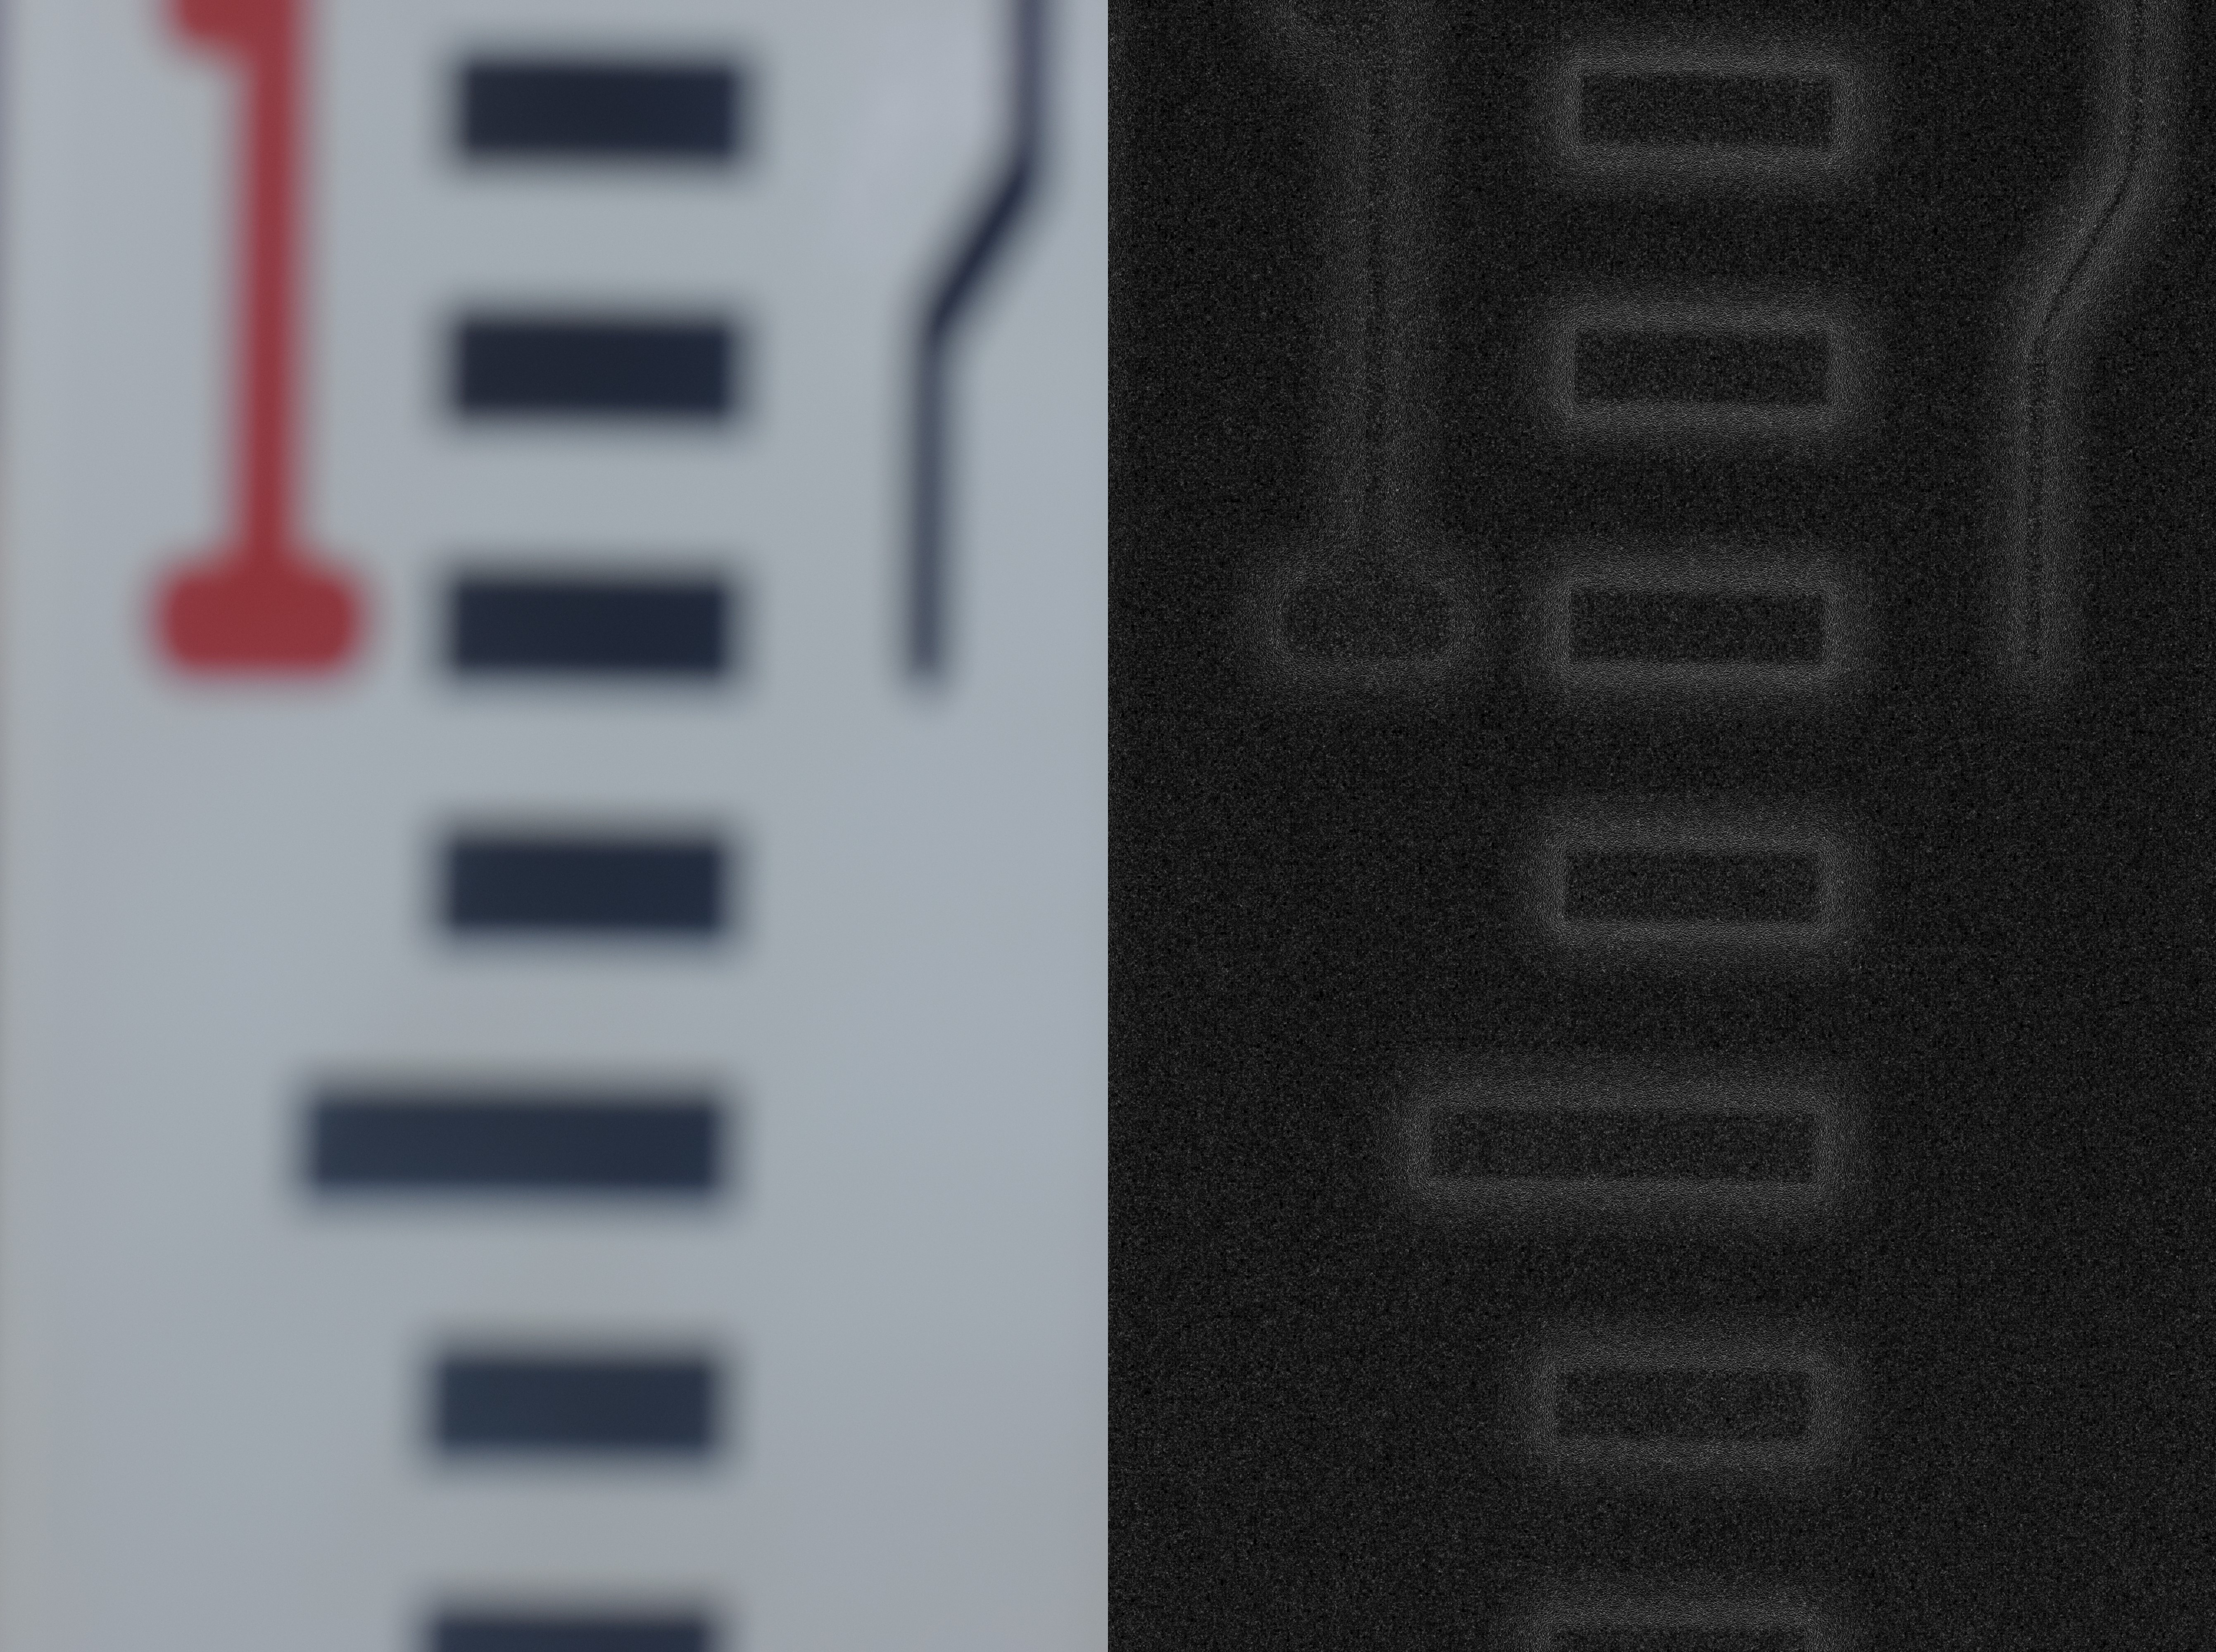
\includegraphics[width=6cm,height=3cm]{25ap=7.1c.jpg} &250.0150449\\
\hline
350 &675341594
 

 & 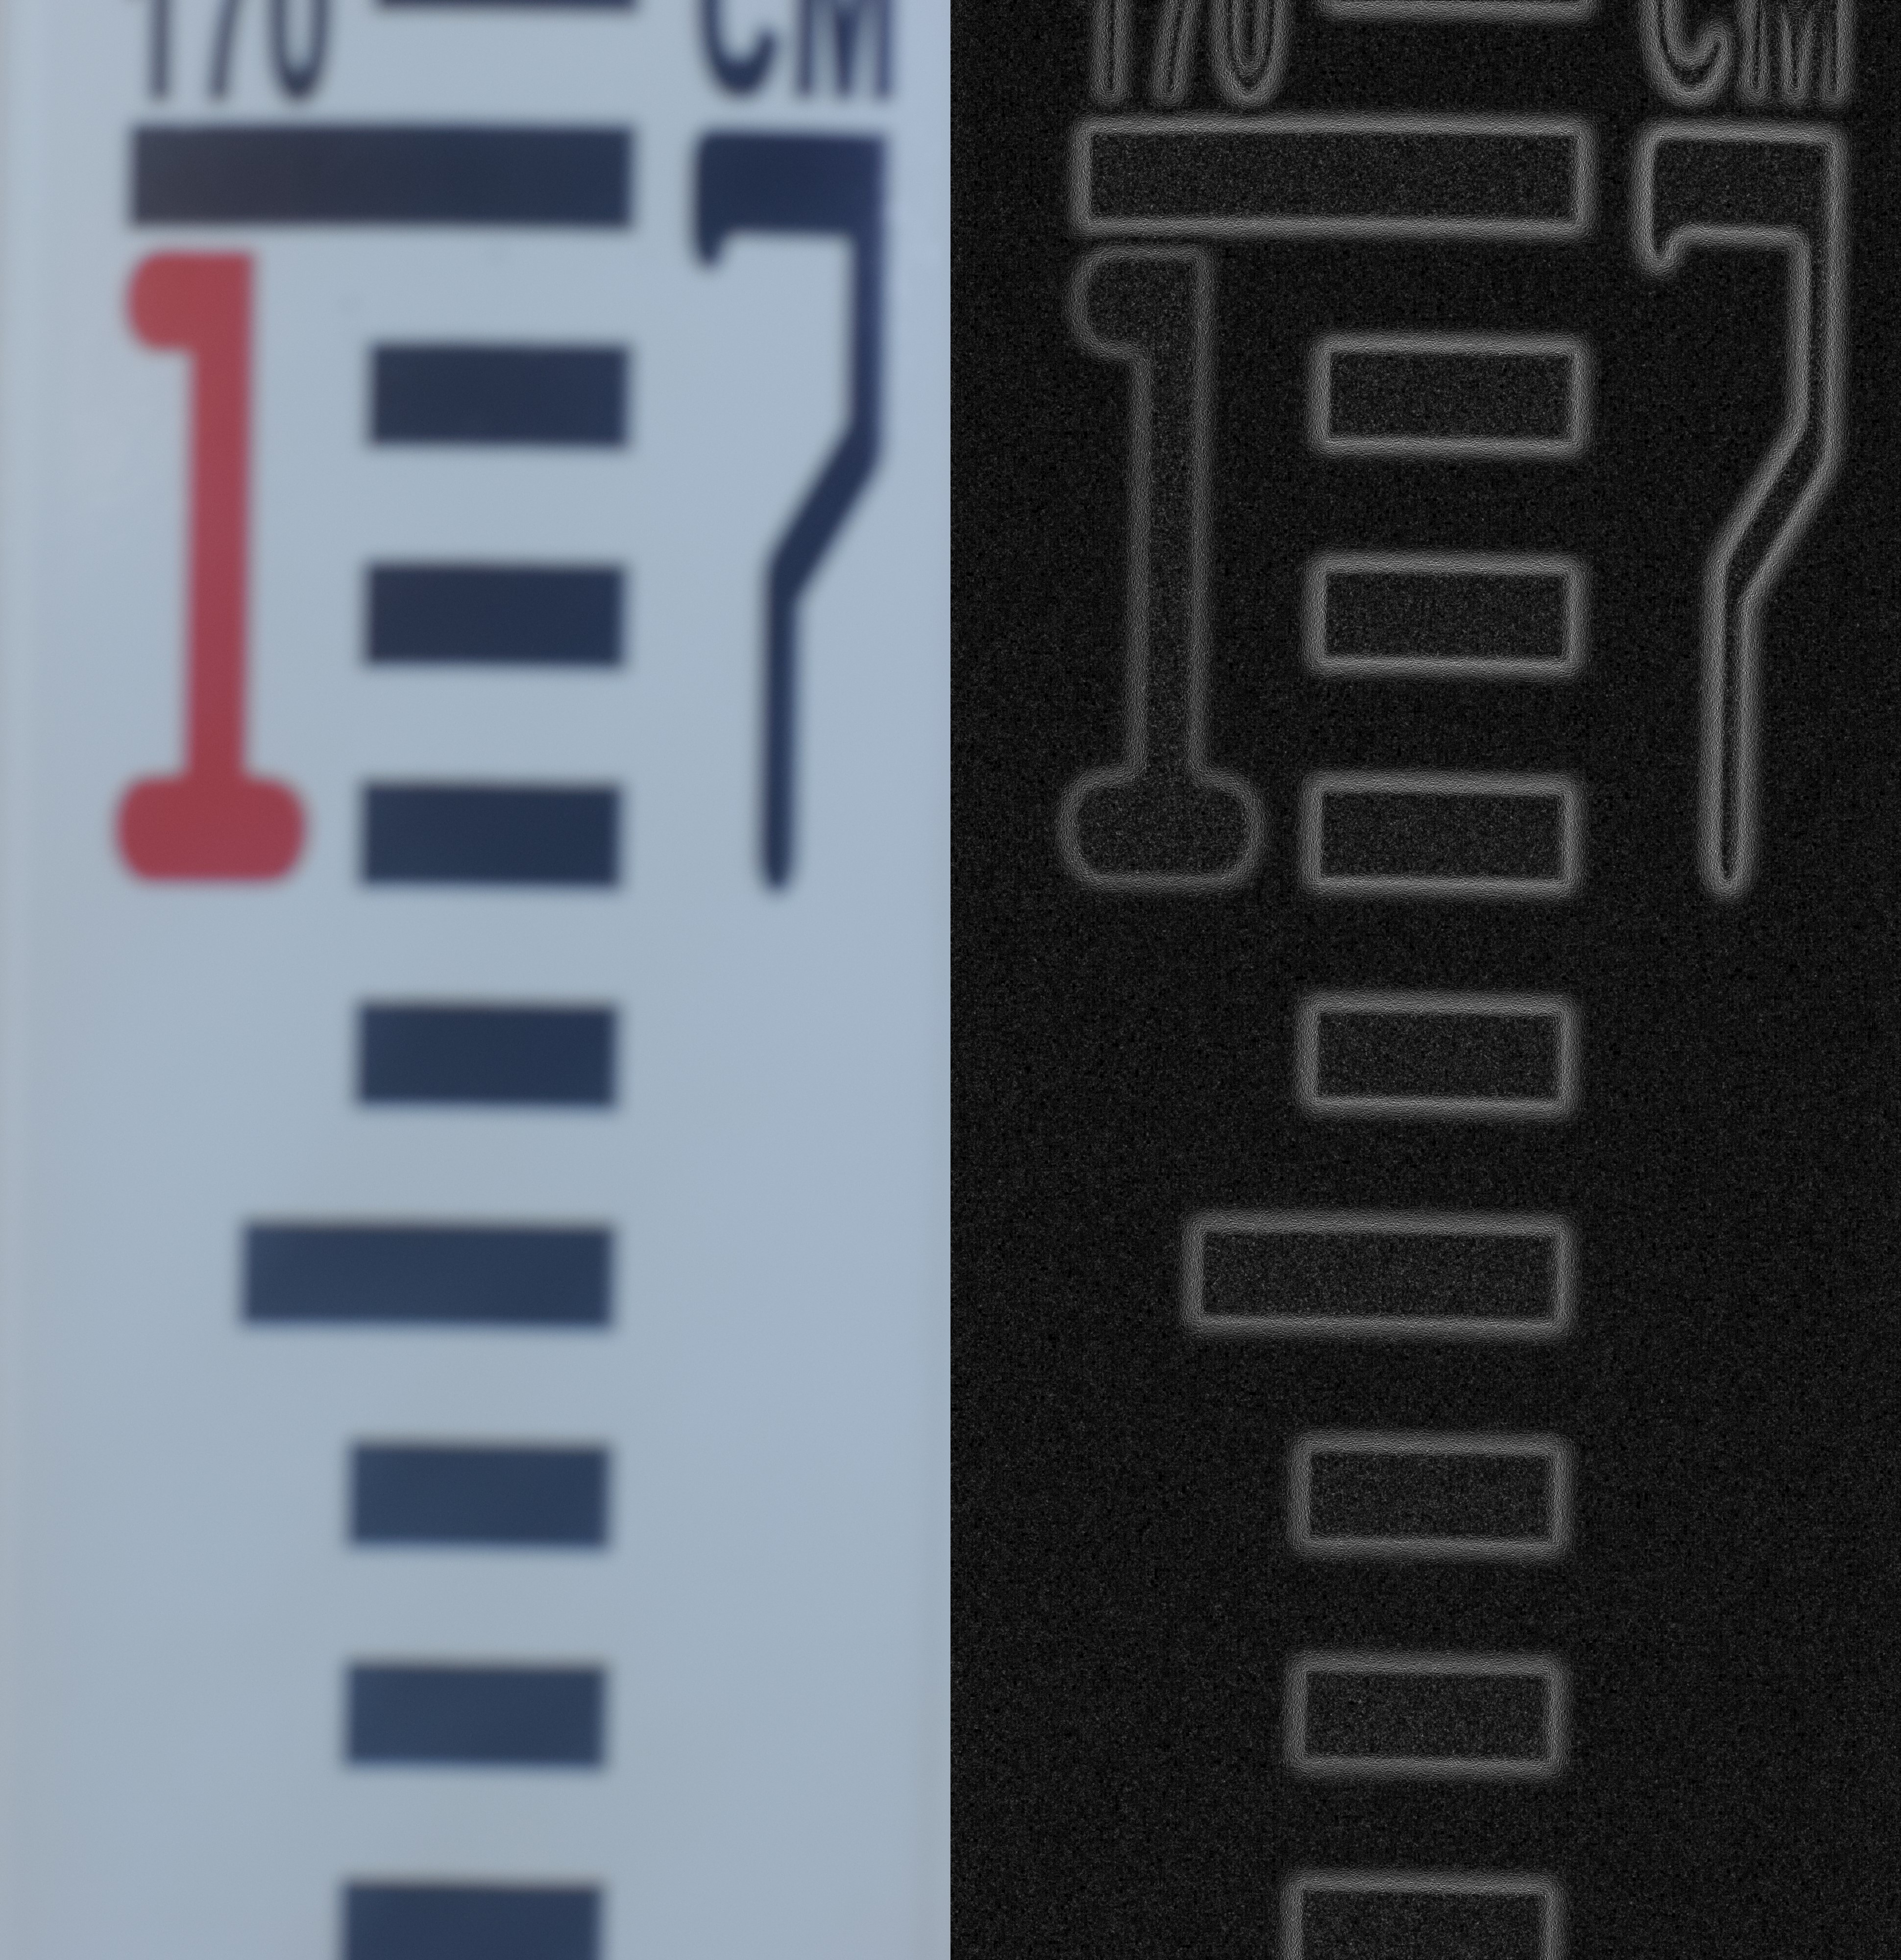
\includegraphics[width=6cm,height=3cm]{35ap=7.1c.jpg}&350.0078543
\\
\hline
450& 1038196086


 & \includegraphics[width=6cm,height=3cm]{45ap=7.1c.jpg}&450.0057096
\\
\hline
550& 475222432


 & \includegraphics[width=6cm,height=3cm]{55ap=7.1c.jpg}&550.0022041
\\
\hline
650 & 347818394


  & \includegraphics[width=6cm,height=2.8cm]{65ap=7.1c.jpg}&649.9997674
\\
\hline
750 &254262442


 & \includegraphics[width=6cm,height=2.8cm]{75ap=7.1c.jpg}&749.9974948
\\
\hline
 \end{tabular}}
\end{table}

\begin{table}[!htbp]
 \caption{sample photographs with aperture=7.1mm at focus =0.6mts} \label{tab:am2}
 f=5cm\\
\scalebox{0.95}{
  \begin{tabular}
{ l l l l }\hline Act dist&  T(d) & Figure & Predicted distance\\
\hline
300 &530200070


 & 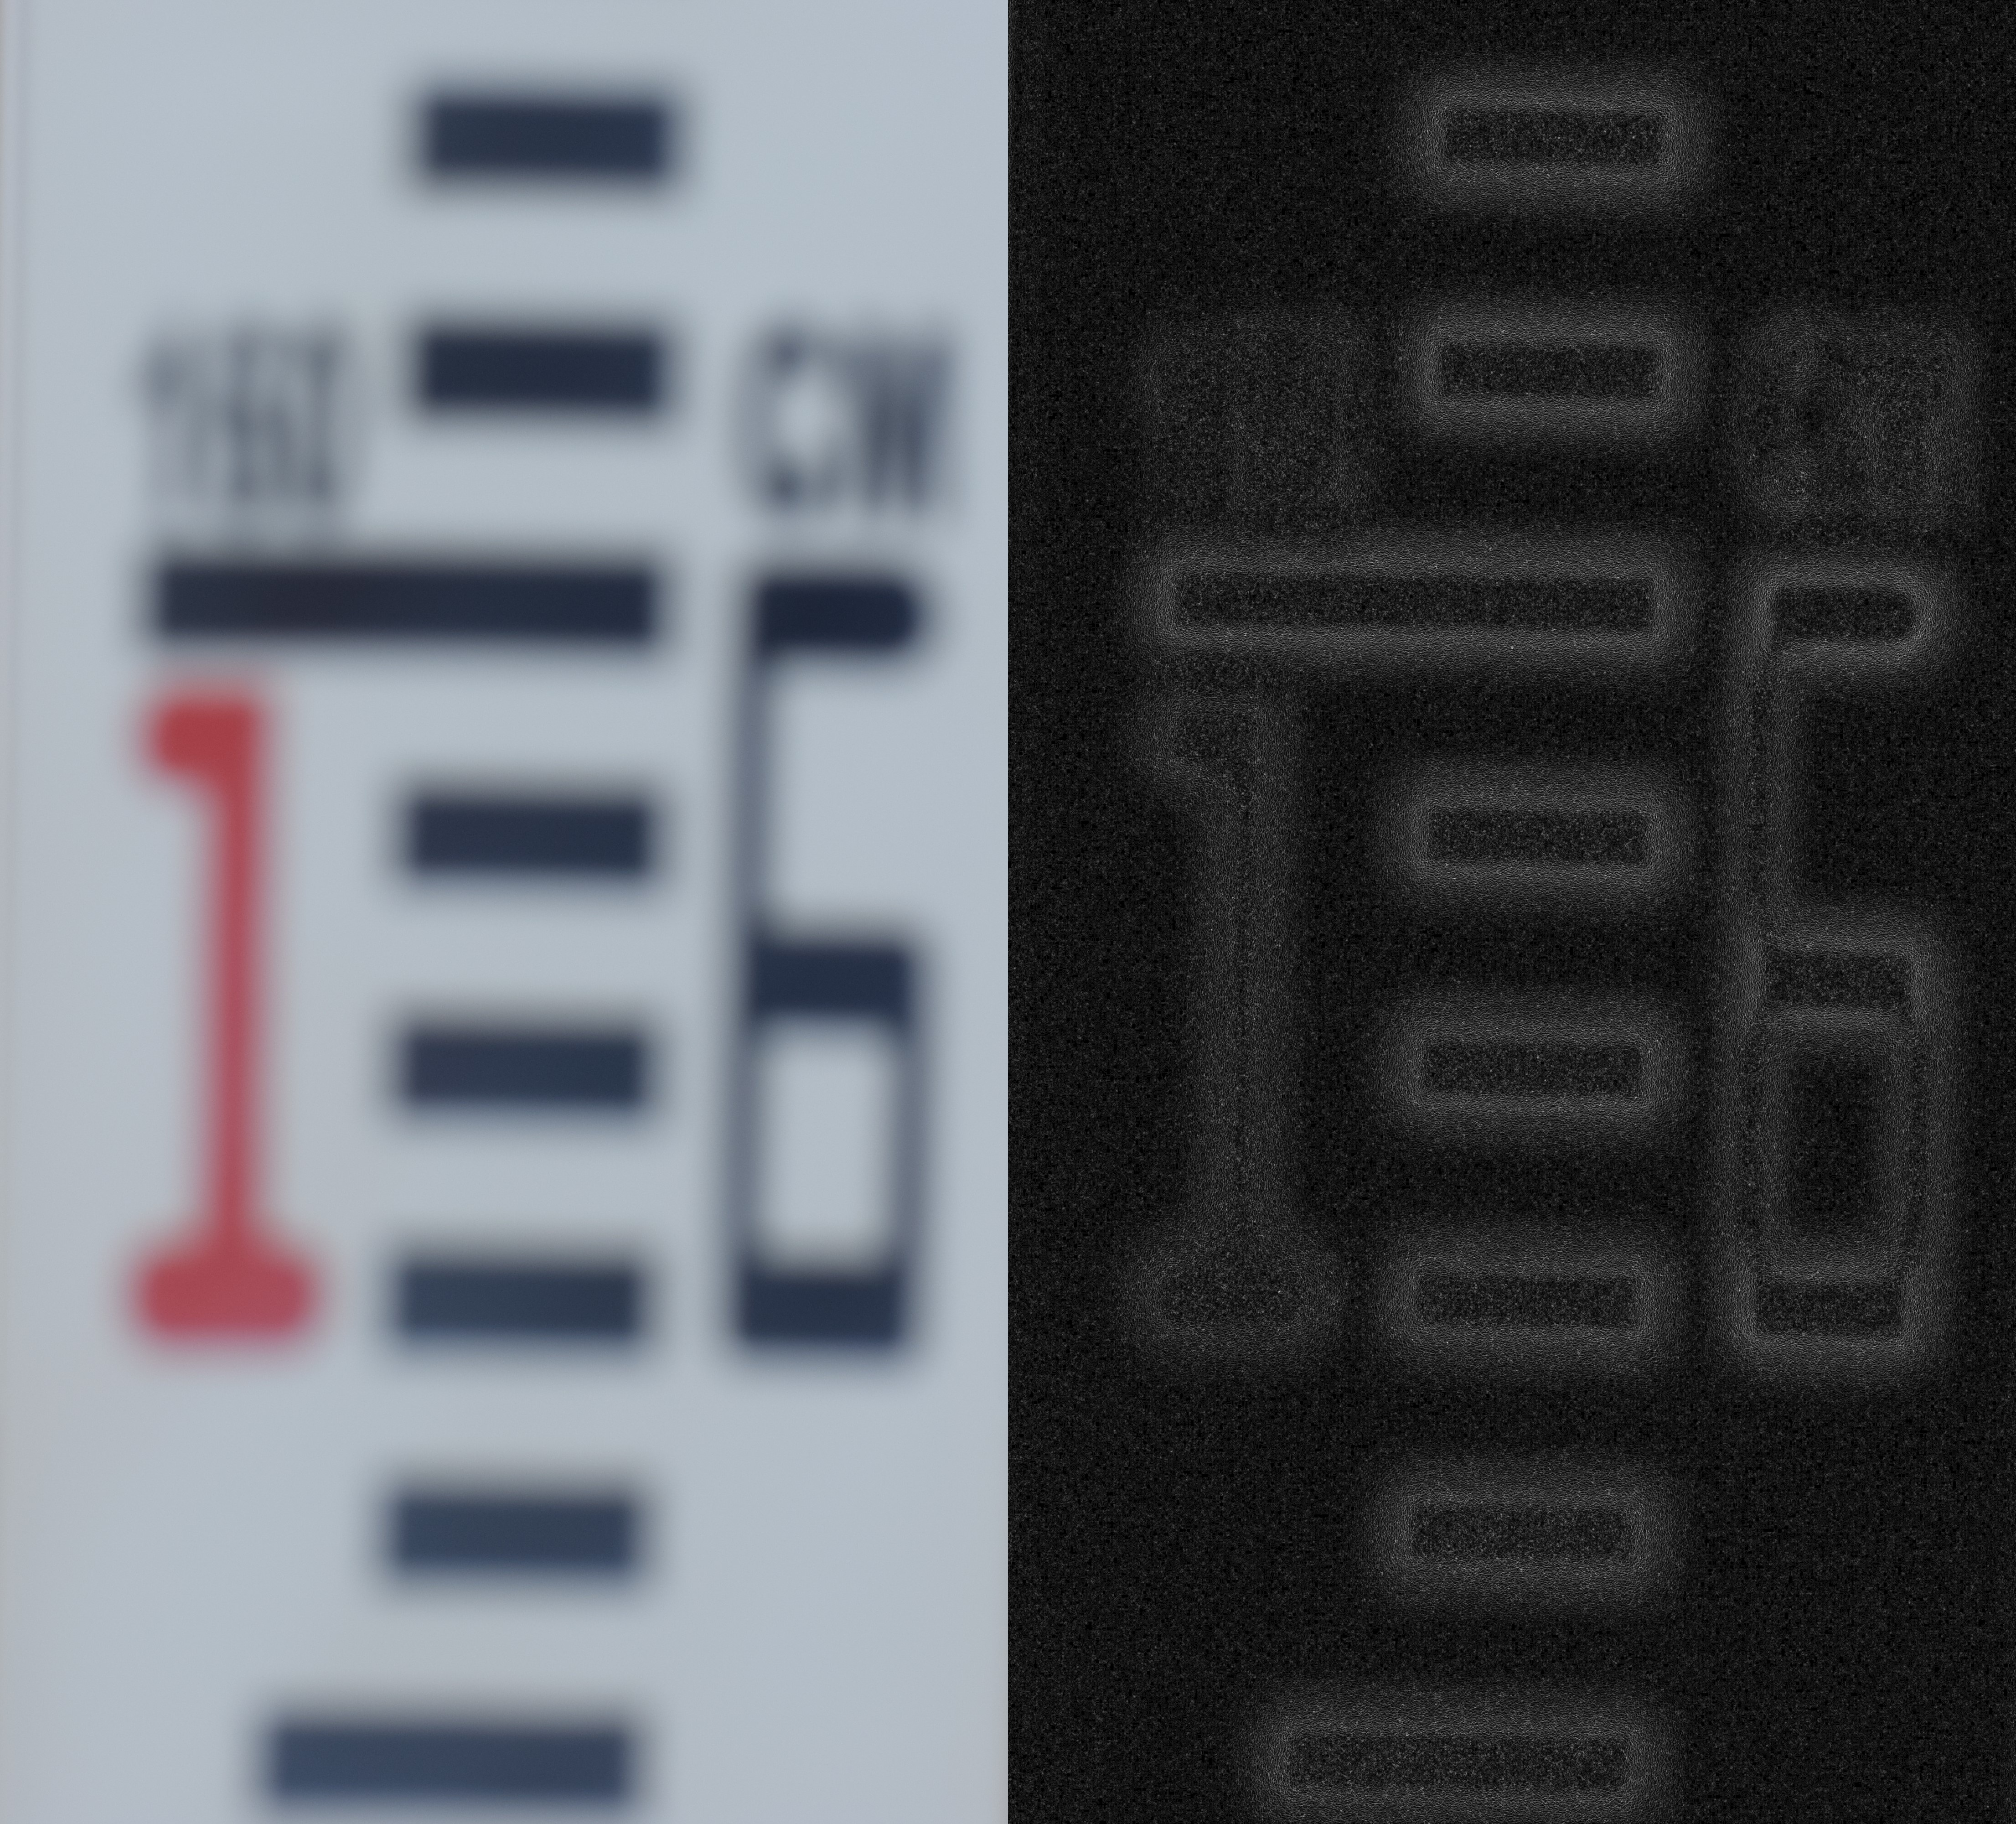
\includegraphics[width=6cm,height=2.5cm]{30ap=7.1c.JPG}&300.0109375
\\
\hline
400 &595258270


 & \includegraphics[width=6cm,height=2.5cm]{40ap=7.1c.JPG}&400.0068504
\\
\hline
500& 1093838306


& \includegraphics[width=6cm,height=2.5cm]{50ap=7.1c.JPG}&500.0037329
\\
\hline
600& 1646652204

 & \includegraphics[width=6cm,height=2.5cm]{60ap=7.1c.JPG}&600.0004818
\\
\hline
700& 795148960

  & \includegraphics[width=6cm,height=2.5cm]{70ap=7.1c.JPG}&699.9988592
\\
\hline
800 & 560742876


& \includegraphics[width=6cm,height=2.3cm]{80ap=7.1c.JPG}&799.995605
\\
\hline
900 &385216040


 & \includegraphics[width=6cm,height=2.3cm]{90ap=7.1c.JPG}&899.9920985
\\
\hline
 \end{tabular}}
\end{table}
\begin{table}[!htbp]
  \caption{sample photographs with aperture=7.1mm at focus =0.8mts} \label{tab:am3}
 f=5cm\\ 
\scalebox{0.95}{
  \begin{tabular}
{ l l l l }\hline Act dist &  T(d)
 & Figure & Predicted distance\\
\hline
500 &428692958

&\includegraphics[width=6cm,height=2.3cm]{50ap=7.1cc.JPG}&500.0037329
\\
\hline
600 &499890598

 & \includegraphics[width=6cm,height=2.5cm]{60ap=7.1cc.JPG}&600.0004818
\\
\hline
700& 1033485664


 & \includegraphics[width=6cm,height=2.5cm]{70ap=7.1cc.JPG}&699.9988592
\\
\hline
800&2100356826


& \includegraphics[width=6cm,height=2.5cm]{80ap=7.1cc.JPG}&799.995605
\\
\hline
900 & 1602901246

 

  & \includegraphics[width=6cm,height=2.5cm]{90ap=7.1cc.JPG}&899.9920985
\\
\hline
1000 &1279292982


 & \includegraphics[width=6cm,height=2.3cm]{100ap=7.1cc.JPG}&999.9883847
\\
\hline
1100 &719627224


 & \includegraphics[width=6cm,height=2.3cm]{110ap=7.1cc.JPG}&1099.983534
\\
\hline
 \end{tabular}}
\end{table}
%\begin{table}[!htbp]
% \caption{sample photographs with f-stop=1.8mm at focus =3mts} \label{tab:am4}
 %f=5cm\\ 
%\scalebox {0.7}{
%  \begin{tabular}
%{ l l l l }\hline Act dist&  $b_{fs}$(cms)  & Figure\\
%\hline
%270 &0.1056 & \includegraphics[width=6cm,height=4cm]{mfb22.jpg}\\
%\hline
%280 &0.0978 & \includegraphics[width=6cm,height=4cm]{mfb23.jpg}\\
%\hline
%290& 0.0959& \includegraphics[width=6cm,height=4cm]{mfb24.jpg}\\
%\hline
%300& 0.0908 & \includegraphics[width=6cm,height=4cm]{mfb25.jpg}\\
%\hline
%310 & 0.0830  & \includegraphics[width=6cm,height=4cm]{mfb26.jpg}\\
%\hline
%320 & 0.0783 & \includegraphics[width=6cm,height=4cm]{mfb27.jpg}\\
%\hline
%330 & 0.0744 & \includegraphics[width=6cm,height=4cm]{mfb28.jpg}\\
%\hline
% \end{tabular}}
%\end{table}

\section{Results and  Interpretations}
The images are taken at different distances at fixed intervals, based on the interpretation of the inverse relationship between the Tenengrad score and the blurriness, for each focus over a range of aperture values. And then, the Tenengrad score is calculated for each image.  RFR (Random Forest Regressor) is being trained using ratios chosen (80\% for the training set and 20\% for the test) on 393 images for focus 45, 60, and 80 with varying apertures (1.8-16 mm) to produce predicted depth, as seen in Algorithm~\ref{alg:Alg2}. To predict the distance, the Random Forest Regressor functions from the Scikit-learn library are trained with the following inputs: \lq Focus range\rq, \lq Aperture\rq, \lq Tenengrad score (T(d))\rq \hspace{.1cm}. A 16GB RAM-equipped Intel(R) Core(TM)-i5 9500 CPU is being used to implement the algorithm. Python code is used to implement the Google colab and jupyter notebook framework. Details about the hardware and software are included in Table \ref{tab:am8}.
The predicted findings obtained from  Algorithm~\ref{alg:Alg2}, are tabulated in Table \ref{tab:am9}.
\pagebreak

\begin{algorithm}
\caption{Predict\textunderscore Distance\textunderscore from Tenengrad score .}
\label{alg:Alg2}
\textbf{Inputs:}$Act_{dist}$,$D_{i=1 \ to \ 3}$,Focus\textunderscore Range,
T(d), aperture. 

\textbf{Outputs:},$Pred_{dist}$(cms)

\textbf{Initalize TrainingParams:}

test\textunderscore size=0.2,iteration(k)=100,

,activaltion=relu,learning rate\textunderscore\\ init=0.1,alpha=0.9, loss= $\leq$ ls $\leq$ ,early\textunderscore stopping=true
 
\textbf{Steps:}

	1 X $\leftarrow$ Extract\textunderscore features \textunderscore  from \textunderscore Dataset($D_{i=1 to 3}$),
	
	2 y $\leftarrow$ Extract\textunderscore Label from \textunderscore Dataset($Actdist_{i=25 to 110}$) 
	
		//splitting of data
		
	3.$Train_{X}$,$Test_{X}$,$Train_{y}$,$Test_{y}$ $\leftarrow$ split(X,y,test\textunderscore size=0.2)

	//Training of model
	
	4 \textbf{for} i=1 to K do
	
	5 rf\_model $\leftarrow$ Random Forest Regressor model trained on ($Train_{X}$,$Train_{y}$)
	
	6 \textbf{EndFor}
	
	7 pred $\leftarrow$ predict($Test_{X}$)
	
	8 Evaluate  RMSE,r
	
	9 actual distance $\leftarrow$ $Test_{y}$
	
	10 Predicted distance $\leftarrow$ pred
	
	11 Focus\textunderscore Range $\leftarrow$ Dataset($D_{1}$)
	
	12 T(d)$\leftarrow$ Dataset($D_{2}$)
	
    13 aperture $\leftarrow$ Dataset($D_{3}$)
	\end{algorithm}
	
\begin{table}[t]
	\caption{Details about the hardware and software used in the workspace.}
	\label{tab:am8}
	  \centering
		 \begin{tabular} {|l l |}
		  \hline
		    Devices & values \\
		   \hline
		    Processor & Intel(R)Core(TM)-i5 9500 CPU @3.00GHz \\
		   \hline
		    Installed RAM & 16.0 GB \\
		   \hline
		    System Type & 64-Bit Operating System,x64-Based Processor\\
		   \hline
		    Software Used &  Microsoft-Excel, google collab,jupyter notebook.\\
		   \hline
		    ML Package Used & OpenCV-V3.9 ,Scikit-learn 0.23-0.24,Python-V3.9.\\
			 \hline
     \end{tabular}
	\end{table}
	
\begin{table}[ht]
\centering
\caption{Predicted camera-to-object distance for a specific focus range, ${\text{Aperture}}$ and Tenengrad Score.}
\label{tab:am9}
\begin{tabular}{|c|c|c|c|c|c|c|}
\hline
\textbf{S.No} & \textbf{Act dist} & \textbf{Pred dist} & \textbf{Focus range} & ${\textbf{Aperture}}$ & ${\textbf {Tenengrad Score}}$  \\ \hline
1 & 250 & 250.0150449
 & 450 & 1.8 &511879910
 \\ \hline
2 & 300 & 300.0109375



 & 600 & 2 & 313273398
 \\ \hline
3 & 350 & 350.0078543
 & 450 & 2.2 & 370398782
 \\ \hline
4 & 400 & 400.0068504
 & 600 & 2.5 & 253223554
 \\ \hline
5 & 450 & 450.0057096
 & 450 & 2.8 & 1028554616
 \\ \hline
6 & 500 &500.0037329
 & 800 & 3.2 &295768310
 \\ \hline
7 & 550 & 550.0022041
 & 450 & 3.5 & 291058134
\\ \hline
8 & 600 & 600.0004818
 & 800 & 4 & 332577218
 \\ \hline
9 & 650 & 649.9997674
 & 450 & 4.5 & 341184826
 \\ \hline
10 & 700 & 699.9988592
 & 800 & 5 & 875533358
 \\ \hline
11 & 750 & 749.9974948
 & 450 & 5.6 & 249112218
 \\ \hline
12 & 800 & 799.995605
 & 800 & 6.3 & 1752501574
\\ \hline
13 & 900 & 899.9920985
 & 800 & 7.1 & 1602901246
 \\ \hline
14 & 1000 & 999.9883847
 & 800 & 8 & 1568996238
 \\ \hline
15 & 1100 & 1099.983534
 & 800 & 9 & 998090620
 \\ \hline
\end{tabular}
\end{table}


Similarly, various other Machine Learning algorithms such as Gradient Boosting Regressor( GBR), Multi-Layer Perceptron ( MLP) Regressor, and XG Boost are also trained on datasets containing features such as Tenengrad score, focus, and aperture in order to predict the object distance w.r.t model. The performance of each model is evaluated using goodness-of-fit metrics like Correlation Coefficient \lq R \rq, Coefficient of Determination \lq R$^{2}$ \rq, \lq Adjusted(R$^{2}$)\rq to ensure it can accurately predict the distance. These metrics assess how well a model explains or predicts the variability of the target variable based on the input features. The mathematical definitions  for these metrics are as follows:


\textbf{Definition 1}: Correlation Coefficient (R)  is used to understand the strength and direction of the relationship between predicted and actual values.
The correlation coefficient $R$ is defined as:
$$
R=\frac{\sum_{i=1}^n\left(y_i-\bar{y}\right)\left(\hat{y}_i-\overline{\hat{y}}\right)}{\sqrt{\sum_{i=1}^n\left(y_i-\bar{y}\right)^2 \sum_{i=1}^n\left(\hat{y}_i-\overline{\hat{y}}\right)^2}}
$$
where:
$y_i$ is the actual value.
$\hat{y}_i$ is the predicted value.
$\bar{y}$ is the mean of the actual values.
$\overline{\hat{y}}$ is the mean of the predicted values.
$n$ is the number of observations.\\


\textbf{Definition 2}: Coefficient of Determination \lq R$^{2}$ \rq indicates the proportion of the variance in the target variable that is explained by the model.\\
The coefficient of determination $R^2$ is defined as:
$$
R^2=1-\frac{\mathrm{SS}_{\mathrm{res}}}{\mathrm{SS}_{\text {tot }}}
$$
where:
$\mathrm{SS}_{\text {res }}$ (Residual Sum of Squares) is:
$$
\mathrm{SS}_{\text {res }}=\sum_{i=1}^n\left(y_i-\hat{y}_i\right)^2
$$
$\mathrm{SS}_{\text {tot }}$ (Total Sum of Squares) is:
$$
\mathrm{SS}_{\mathrm{tot}}=\sum_{i=1}^n\left(y_i-\bar{y}\right)^2
$$\\



\textbf{Definition 3}: \lq Adjusted(R$^{2}$)\rq provides a more accurate measure of model performance by adjusting R2 for the number of predictors, accounting for potential over-fitting.\\
The adjusted $R^2$ is defined as:
$$
\text { Adjusted } R^2=1-\left(\frac{1-R^2}{n-k-1}\right)(n-1)
$$
where:
$R^2$ is the coefficient of determination.
$n$ is the number of observations.
$k$ is the number of independent variables (predictors).\\


In this context, we have taken k as 3, namely Focus, Aperture, and Tenengrad score, \lq n\rq \space is taken as 393, and the target variable to be predicted is the object distance ( or depth) w.r.t to the camera.\\

The performance evaluation is done for each ML model trained using the metrics as mentioned above and are tabulated in Table  \ref{tab:modeleva}. 
\begin{table*}[!htbp]
\centering
\caption{Model Evaluation for Camera to Object Distance Predicted and Graph Visualization of Inverse Relationship Between Predicted Distance vs Tenengrad Score}
\label{tab:modeleva}
\begin{tabular}{ c c c c c }
\hline 
S.No. & ML Model & R & R\textsuperscript{2} & Adjusted R\textsuperscript{2} \\
\hline
1 & Random Forest & 1 & 1 & 1 \\
\hline
2 & Gradient Boosting Regressor & 0.999999 & 0.999999 &  0.999999 \\
\hline
3 & MLP Regressor &0.999999 & 0.999730 &0.999723 \\
\hline
4 & XGBoost &0.999999 &0.999999 & 0.999999 \\
\hline
\end{tabular}
\end{table*}


In Table \ref{tab:modelinv1} and Table \ref{tab:modelinv2}, the predicted distance derived from the model(s) under evaluation is displayed against the Tenengrad score feature for each of the focus points, 45.60 and 80 separately.  It is evident from the graphs' interpreted that the score value tends to decrease as we move farther from the fixed focus (let's say 45, 60, or 80). This exhibits non-linearity between the predicted distance and the Tenengrad score value wrt to the camera focus distance.   Specifically, it resembles a curve with a peak, which can often be modeled by a polynomial function. A polynomial function of degree 2 or higher could capture this behavior. For instance, a quadratic function (polynomial of degree 2) might fit the data well and exhibit a parabolic shape, where the score increases to a maximum point and then decreases. In summary, the curve is likely non-linear and polynomial, with a peak where the score value reaches its maximum. This peak point represents the focus point( or focal distance) at which the image remains in focus. From that point on, a fall in the Tenengrad score value is observed anytime the object goes down the curve from either.



\begin{table*}[!htbp]
\caption{Visualization of  curves depicting the relationship between Predicted Distance and Tenengrad Score w.r.t to Focus Point (or Focus Distance)} 
\label{tab:modelinv1}
\centering 
\begin{tabular}{ c c c c }\hline  
focus&Random Forest & Gradient Boosting Regressor \\
\hline
\hline
45& \includegraphics[width=5cm,height=5.5cm]{rf45.JPG} & \includegraphics[width=5cm,height=5.5cm]{gbr45.JPG} \\
\hline
60 & \includegraphics[width=5cm,height=5.5cm]{rf60.JPG} & \includegraphics[width=5cm,height=5.5cm]{gbr60.JPG} \\
\hline
80 & \includegraphics[width=5cm,height=5.5cm]{rf80.JPG} & \includegraphics[width=5cm,height=5.5cm]{gbr80.JPG} \\
\hline

\end{tabular}
\end{table*}



\begin{table*}[!htbp]
\caption{Visualization of inverse relationship between Predicted Distance and Tenengrad Score w.r.t to Focus Point (or Focus Distance).} 
\label{tab:modelinv2}
\centering 
\begin{tabular}{ c c c c }\hline  
focus&MLP Regressor& XG BOOST \\
\hline
\hline
45&  \includegraphics[width=5cm,height=5.5cm]{mlp45.JPG} &
\includegraphics[width=5cm,height=5.5cm]{xgb45.JPG}\\
\hline
60  & \includegraphics[width=5cm,height=5.5cm]{mlp60.JPG}  &
\includegraphics[width=5cm,height=5.5cm]{xgb60.JPG}\\
\hline
80 &\includegraphics[width=5cm,height=5.5cm]{mlp80.JPG} &
\includegraphics[width=5cm,height=5.5cm]{xgb80.JPG}  \\
\hline

\end{tabular}
\end{table*}
\pagebreak

\pagebreak

\subsection{\textsf{Method validation}}
In order to validate the  Random Forest Regressor model trained on the dataset with features such as Focus, Aperture, and Tenengrad score, the dataset is split into 5 subsets of approximately equal size. The model is trained on 4 of these subsets (called training folds) and evaluated on the remaining subset (called the validation fold). This process is repeated 5 times, each time using a different subset as the validation fold and the remaining 4 subsets as the training data. The procedure is explained in Algorithm~\ref{alg:Alg3}. The The performance metrics (cross validation scores R$^{2}$), Mean R$^{2}$, Cross-Validation Adjusted R$^{2}$, Mean Adjusted R$^{2}$, Cross-Validation RMSE, Mean RMSE Scores are calculated for each of the 5 validation folds and are tabulated in  Tables \ref{tab:Validate}



\begin{algorithm}
\caption{Random Forest Regression with K-Fold Cross-Validation}
\label{alg:Alg3}
\begin{algorithmic}[1]
\Require Dataset $(X, y)$, number of folds $k$, random seed $s$, number of estimators $n\_estimators$
\Ensure Mean R\textsuperscript{2} score, Mean Adjusted R\textsuperscript{2} score, Mean RMSE score

\State Load dataset
\State $X \gets$ Features from dataset
\State $y \gets$ Target variable from dataset

\State Split data into training set $(X_{train}, y_{train})$ and testing set $(X_{test}, y_{test})$ using \texttt{train\_test\_split} with $test\_size=0.2$ and $random\_state=s$

\State Initialize Random Forest Regressor with $n\_estimators$ and $random\_state=s$
\State Train Random Forest Regressor on $(X_{train}, y_{train})$

\State Initialize K-Fold cross-validation with $n\_splits=k$, $shuffle=\text{True}$, and $random\_state=s$

\State Perform cross-validation using R\textsuperscript{2} as the scoring metric and store scores in $cv\_r2\_scores$

\State \textbf{Output} Cross-Validation R\textsuperscript{2} Scores and Mean R\textsuperscript{2} Score

\State Initialize array $adjusted\_r2\_scores$

\For{each split $i$ in $k$ folds}
    \State Split data into $(X_{train\_fold}, y_{train\_fold})$ and $(X_{test\_fold}, y_{test\_fold})$
    \State Train Random Forest Regressor on $(X_{train\_fold}, y_{train\_fold})$
    \State Predict $y\_pred\_fold$ on $X_{test\_fold}$
    \State Calculate R\textsuperscript{2} score $r2\_fold$ for fold $i$
    \State Calculate Adjusted R\textsuperscript{2} score $adjusted\_r2\_fold$ using:
    \[
    adjusted\_r2\_fold = 1 - \left(\frac{(1 - r2\_fold) \times (n - 1)}{(n - k - 1)}\right)
    \]
    \State Store $adjusted\_r2\_fold$ in $adjusted\_r2\_scores$
\EndFor

\State \textbf{Output} Cross-Validation Adjusted R\textsuperscript{2} Scores and Mean Adjusted R\textsuperscript{2} Score

\State Define RMSE scorer using \texttt{make\_scorer}
\State Perform cross-validation using RMSE as the scoring metric and store scores in $cv\_rmse\_scores$

\State \textbf{Output} Cross-Validation RMSE Scores and Mean RMSE Score

\end{algorithmic}
\end{algorithm}

\begin{table*}[!htbp]
\caption{Cross-Validation Performance Metrics for Random Forest Regressor.} 
\label{tab:Validate}
\centering 

\begin{tabular}{|l|l|l|l|}  % Add the missing '|' at the end
\hline 
Fold & $R^2$ Score & Adjusted $R^2$ Score & RMSE \\
\hline 
1 & 1.0 & 1.0 & $8.70383371 \times 10^{-13}$ \\
\hline 
2 & 1.0 & 1.0 & $8.78335660 \times 10^{-13}$ \\
\hline 
3 & 1.0 & 1.0 & $8.95764837 \times 10^{-13}$ \\
\hline 
4 & 1.0 & 1.0 & $8.94245048 \times 10^{-13}$ \\
\hline 
5 & 1.0 & 1.0 & $8.81437298 \times 10^{-13}$ \\
\hline 
Mean & 1.0 & 1.0 & $8.840332428116105 \times 10^{-13}$ \\
\hline

\end{tabular}
\end{table*}
\begin{table*}[!htbp]
% table caption is above the table
\caption{Model evaluation: Discusses the present works' prototype, methodology, and advancement.}
\label{tab:blurrcomp}       % Give a unique label
% For LaTeX tables use
\scalebox {0.75}{
\begin{tabular}{p{20mm}p{40mm}p{40mm}p{20mm}p{20mm}}
\hline\noalign{\smallskip}
S.No.&\textbf{Experimental set-up } & \textbf{Technique} & \textbf{Act (Range in mts)} & \textbf{Performance metric}\\

\noalign{\smallskip}\hline\noalign{\smallskip}
1 & C.Q. Farias et al.\textit{\cite{bib5}} (2016). parallel stereo system mount configuration using two identical cameras.
 & Triangulation method & 2.79-8.3 & RMSE=0.667 \\
2 & Said Pertuza et al.\textit{\cite{bib11}} (2018). & Focus-based & 0.2–1.6 & r = 5cm \\
3 & Monteiro et al.\cite{bib8} (2018) \& Palmieri et al.\textit{\cite{bib9}} (2019). Taking into account: the sensor, primary lens, and microlens array. & Light Field Refocusing & 0.2-1.6 & r = 0.99 \\
4 & Alphonse et al.\textit{\cite{bib10}} (2021). Depth Estimation Technique with Nikon D5300, Nikkor AF-S 50 mm prime lens camera. & \text Relationship in inverse between object depth and object size.[ & 0.5-1.1 & r = 0.99213 \\
5 & Keshri et al.\textit{\cite{bib12}} (2023). Proposed Method with DSLR
Nikkor 50 mm primary camera.& \text The cubic relationship between focus and object depth, and the inverse relationship between lens blurrstrain $b_{fs}$ and object depth. & 0.5-3.3 & r=0.987\\

6 & Proposed Method  (\textbf{Single RGB camera}). & \textbf{A parabolic relationship between Tenengrad score T(d) and object distance (or depth)}  with peak representing the focus point.   & 0.25-1.1 & r = 0.9999 \\
\noalign{\smallskip}\hline\noalign{\smallskip}

\end{tabular}}

\end{table*}

\subsubsection{Influence of Predicted Distance on Tenengrad Score for different focus settings }

Given the influence of predicted distance on the Tenengrad score  as shown in Table  \ref{tab: Focus-score} different focus settings, here's an analysis:

\begin{table*}[!htbp]
\caption{Impact of Predicted distance on Tenengrad Score for different focus points ( or focus distances(s).} 
\label{tab: Focus-score}
\centering 

\begin{tabular}{|l|l|l|}  % Add the missing '|' at the end
\hline 
S.No & Focus &  Score  \\
\hline 
1 & 45 &  0.5173273775698527 \\
\hline 
2 & 60 & 0.4951133528232609 \\
\hline 
3 & 80 &  0.5160461641214248 \\
\hline 
\end{tabular}
\end{table*}

Interpreting the score trends for focus distances 45,60 and 80, it is understood that there is a slight decrease in the Tenengrad score when the focus is at 60 compared to 45, and the score value returns close to the value at focus 45 when the focus is at 80. The score at Focus 60 is lower than at Focus 45 and Focus 80, suggesting a potential local minimum in performance. This implies that Focus 60 might not be as optimal as the other focus settings for achieving a higher Tenengrad score. Concerning stability at extremes. The Tenengrad score remains relatively stable at the extreme focus values (45 and 80), indicating that either of these might be preferable depending on other factors or specific requirements. \\

The aforementioned findings suggest that, to acquire stable Tenengrad scores and accurately predict the object distance in connection with the focus point, it is always preferable to set the camera to either focus 45 or 60.\\

\subsubsection{Comparative Analysis wrt to existing procedures and findings of Depth estimates from single RGB image}
The analogy is predicated on precision, technology, and experimental arrangement. Table \ref{tab:blurrcomp} illustrates the high degree of consistency (r) using a Pearson's correlation between the quoted (actual) and intended (approximated) depth values coefficient of 1.0. that our method achieves, beating the depth estimate technique(s) of Yujiao et al. (2016) \cite{bib4} and Sanchez-Ferreira et al. (2016) \cite{bib5}.

Unlike the primary lens and micro-lens setups explained in Palmieri et al. (2019) \cite{bib9} and Said Pertuz et al. (2018) \cite{bib11}, One DSLR Nikkor 18-55 mm zoom lens was utilized by us for 2D pictures. Alphonse et al. (2021) \cite{bib10}  determined the depth by linking the object depth with two additional metrics, particularly focal point, gap sweep, and object size in an image plane of the camera, in contrast to the growing gap and length among both picture planes and the microlens. The shapes are then concentrated at 50 mm Nikkor main glasses by gradually altering the entrance  $f_{stop}$ for repeated reading collecting multiple operating ranges starting at 10 cm. The ISO and pinhole motion settings are adjusted to get the necessary proportions for a detector to generate a crisp picture. The auto-focus mode is used for the duration of the experiment. In our instance, An image's blurriness is also taken into account while measuring the depth. Our hypothesis should be able to calculate the degree of blur regardless of whether the camera is in focus or not by using the focal distance. Using Tenengrad metric measurement. the curve is likely non-linear and polynomial, with a peak where the score value reaches its maximum. This maximum ( or peak point) represents the focal distance ( or focal point) at which the image is in focus and from this point either to the left or right side, the Tenengrad score tends to vary in proportion with the amount of blur as we move away from the focal distance in parabolic fashion. This parabolic nature of the curve depicting the relationship between predicted object distance ( or depth) and Tenengrad score quantifying the degree of blur is capable of competing with Alphonse et al.(2021) \cite{bib10}, Felix Sattler (2024) \cite{bib15}, Aolei Yang et al.(2024) \cite{bib14}, and Liman Liu et al.(2024) \cite{bib16}. by offering a higher level of fit quality with an RMSE of 8.604584927025298 $\times$  e$^{-13}$ (extremely small)  on the acquisition of Nikon model data sets for depth estimation up to 3.3 meters.\pagebreak
\subsection{Abbreviations and Symbols }
\subsubsection{Abbreviations: }

\begin{table}[!htbp]
 \caption{Abbreviations Table.} \label{tab:am6}
 
\begin{tabular}
{ l l l l l l}\hline S.No&Abbreviations& Definition \\
\hline
\hline
1&DSLR&Digital Single-Lens Reflex.\\
\hline
2&RMSE&Root-mean-square error.\\
\hline
8&TOF&Time-of-Flight. \\
\hline
9&ISO&International Organization for Standardization.\\
\hline
 \end{tabular}
\end{table}
\subsubsection{ Symbols: }
\begin{table}[!htbp]
 \caption{Symbols Used.} \label{tab:am6b}
 
\begin{tabular}
{ l l l l l l}\hline S.No& Symbol& Definition \\
\hline
\hline
1&$Act_{dist}$&Actual Distance. \\
\hline
2&$T{(d)}$&Tenengrad Score.\\
\hline
3&aperture&The ratio of the lens focal length to the diameter of the entrance pupil.\\
\hline
4&$Pred_{dist}$&Predicted Distance.\\
\hline
5&r&Pearson’s Correlation Coefficient.\\
\hline
6&R&The Coefficient of Multiple Correlation.\\
\hline
7&$R^{2}$&The proportion of the dependent variable's variance.\\
\hline
8&$b_{fs}$&Blurstrain.\\
\hline
9&{$f_{stop}$}&The ratio of the lens focal length to the diameter of the entrance pupil.\\
\hline
 \end{tabular}
\end{table}

\pagebreak
\section{Conclusion}
This study presents the idea of determining the degree of blur using the Tenengrad score and relating the object distance (or depth) to the blurriness. Investigating the profundity (or distance) impacts of object dimensions and of the aperture of the lens in manual focus style is done through close-range photography. It was discovered that a picture's blurriness fluctuates proportionately from the focus point under the true depth information. A requirement for assessing the depth of the item Regarding the focal point is its blurriness. A Nikon D5300 and a 50 mm prime lens are used for testing. The lens is focused to infinite focus to calculate the distance measurements for different apertures.\par

The study developed a parabolic (quadratic) model to describe the relationship between depth and blurriness, with R=1.0, R$^{2}$=1.0 and Adjusted R$^{2}$=1.0,  with negligible Error Estimate in model's predictions in contrast to the Felix Sattler (2024) \cite{bib15}, Aolei Yang et al.(2024) \cite{bib14}, and Liman Liu et al.(2024) \cite{bib16}. The influence of predicted distance on Tenengrad score for different focus settings also proved that camera has to be set to Focus 45 or 80, so that Tenengrad scores at these focus points remains stable gives exactly degree of blur by which object distance can be predicted with negligible error estimates. 

To estimate depth, the suggested methods employed an experimental light field imaging setup with a single lens arrangement. With an RMSE of 0.05 and a correlation of roughly 98.7\%, the depth estimates I obtained from the innovative design approximate the genuine facts better than existing attempts about light and stereo imaging. The work is then compared to the depth estimation technique of Alphonse et al. (2021) \cite{bib10} utilizing just one RGB  photography camera, and it is demonstrated to be effective in calculating depth estimations from blur with 100\% precision, which was not the case in an earlier instance. It is clear that, regardless of whether a picture is in focus or not, our suggested model performs well when calculating depth estimations up to a range of 1.1 meters for both sharp and blurred image(s).

Future Work: It's foreseen that the project will expand to incorporate indoor object movement. Our study will concentrate on determining motion blur as an item moves and utilizing that data to determine depth.

Acknowledgements:
We are deeply grateful to the Southern Indian Cinematographers Association (SICA), Chennai, for their assistance in creating the data set that bolsters the hypothesis that has been put out. The researcher also thanks NIT Trichy's Computer Applications Department and students for their help.\pagebreak

\subsection{Declarations:}

 \lq\lq Funding and/or Conflicts of Interest/Competing interests\rq\rq: Do not have any conflict of interest.
\subsection{Data and Code Availability:}The datasets and Code generated during and/or analysed for the Parabolic Depth Estimation from Image Blur Using Tenengrad Scores with a Single RGB Camera are available from the corresponding author on reasonable request. {\url{https://github.com/keshri9/The-Visual-Computer/tree/main}}

\bibliography{sn-bibliography}

\end{document}